\section{Méthodologie}
\subsection{Agile}

Comme brièvement abordé précédemment, vu la l'envergure et la complexité du projet, j'ai décidé de travailler de manière "agile". Mais qu'est-ce que "l'agilité" dans le monde du développement informatique? \textit{"En ingénierie logicielle, les pratiques agiles mettent en avant la collaboration entre des équipes auto-organisées et pluridisciplinaires et leurs clients1. Elles s'appuient sur l'utilisation d'un cadre méthodologique léger mais suffisant centré sur l'humain et la communication2. Elles préconisent une planification adaptative, un développement évolutif, une livraison précoce et une amélioration continue, et elles encouragent des réponses flexibles au changement"\cite{Agile}}.

\newpara

Concrètement, dans le cadre de ce projet, cela à impliqué que j'ai travaillé de manière incrémentale comme l'illustre la \textit{figure \ref{agile}} ci-dessous. 
\begin{figure}[H]
  \centering
  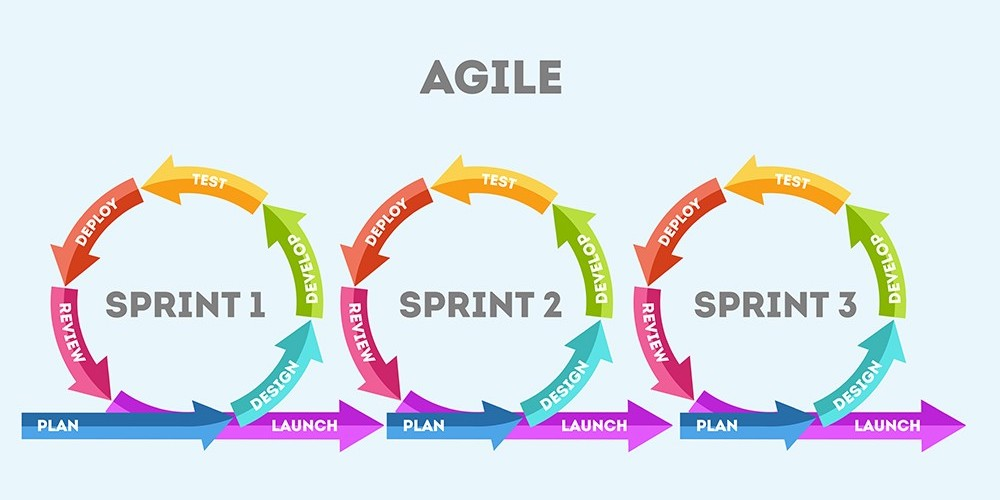
\includegraphics[width=0.75\linewidth]{img/agile.jpeg}
  \caption{ \textit{Les raisons pour utiliser les méthodes Agile en entreprise} de 300\_librarians}
  \label{agile}
\end{figure}
Chaque fonctionnalité de ce projet peut être representée par un "sprint". En d'autres termes j'ai, pour chaque fonctionnalité: 
\begin{enumerate}
  \item détaillé sous forme d'une US (PLAN + DESIGN) 
  \item implémenté (DEVELOP)
  \item testé par le biais de tests automatisé ou manuellement (TEST)
  \item déployé l'ensemble en production (DEPLOY)
  \item demandé un feedback au client (REVIEW)
  \item adapté la fonctionnalité en fonction du feedback 
\end{enumerate} 

\newpara

Cette Méthodologie a été très efficace et a permis une bonne collaboration avec le client. 

\subsection{Choix des technologies}
\subsubsection{Backend}
\begin{figure}[H]
  \begin{minipage}{.3\textwidth}
    
\includegraphics[width=0.75\linewidth]{img/tech/NestJs.png} 
  \end{minipage}
  \begin{minipage}{.7\textwidth}
    \begin{description}
      \item[Framework]: NestJs
      \item[Language]: TypeScript
      \item[Runtime environnement]: NodeJs  
      \item[ORM]: TypeOrm 
    \end{description}
    Tout d'abord, vu l'envergure du projet, il me paraissait important de veiller à une bonne structure et de garder en tête la maintenance du projet au fil du temps. Dans ces circonstances, il est important d'utiliser un framework. Quant au choix du framework, dans un premier temps mon choix s'est porté sur la suite NodeJs-ExpressJs. Ce choix était initialement justifié par le fait que j'avais déjà travailler avec ceux-ci. Après quelques semaines de développement, je me suis rendu compte que je préférait nettement utiliser le TypeScript pour un projet d'une tel envergure. J'ai des lors décidé de changer de framework et ai migré mon application NodeJs-Express vers du NestJs. Le NestJs utilise du Typescript et permet de bien structurer son code comme au frontend avec Angular. (voir ci-après)
  \end{minipage}
\end{figure}

\subsubsection{Frontend}
\begin{figure}[H]
  \begin{minipage}{.3\textwidth}
    
\includegraphics[width=0.75\linewidth]{img/tech/Angular.png}
  \end{minipage}
  \begin{minipage}{.7\textwidth}
    \begin{description}
      \item[Framework]: Angular
      \item[Languages]: \begin{itemize}
        \item TypeScript
        \item HTML
        \item SCSS
      \end{itemize} 
    \end{description}
    Tout comme pour le backend, il est évident que l'utilisation d'un framework est indispensable. Le choix du framework s'est fait sur base de mon expérience personnelle. En effet, durant mes années d'études, j'ai eu l'occasion d'utiliser différent frameworks frontend tel que React, Vue et Angular. J'ai particulièrement bien aimé travailler avec ce dernier car il impose une certaine rigueur tout en restant relativement simple d'utilisation.
  \end{minipage}
\end{figure}

\newpage

\subsubsection{base de données}

\begin{figure}[H]
  \begin{minipage}{.3\textwidth}
    
\includegraphics[width=0.75\linewidth]{img/tech/PostgreSql.png} 
  \end{minipage} 
  \begin{minipage}{.7\textwidth}
    Le choix de la base de données a été motivé par trois critères :
    \begin{enumerate}
      \item \textbf{SQL}: Comme expliqué lors de l'analyse des besoins du client dans la section "base de données", vu le grand nombre de relations entre les différentes données, une base de données SQL est primordiale pour la bonne organisation du système d'information.
      \item \textbf{Notoriété}: PostgreSQL est fortement utilisé dans le milieu proféssionnel ce qui lui oblige d'être mis à jour régulièrement et ce tant au niveau sécurité que en ajout de fonctionnalités. C'est donc une base de données fiable, utilisable à long terme et maîtrisée par de nombreux développeurs.
      \item \textbf{Expérience}: Bien que toutes les bases de données SQL se ressemble, le fait d'avoir déjà manipuler et de s'être familiariser avec PostgreSql m'offre un gain de temps considérable.
    \end{enumerate}
  \end{minipage} 
\end{figure}

\subsubsection{Autre}

\subsubsubsection{API}

Afin de tester les différents endpoints API de l'application, j'ai décidé d'utiliser \textbf{Insomnia}\footnote{\url{https://insomnia.rest}}. Insomnia permet non seulement de tester mon API en temps réel mais permet aussi d'écrire la documentation. Je n'utiliserai néanmoins pas cette dernière fonctionnalité étant donnée que le framework backend (NestJs) que j'utilise me permet de générer automatiquement et facilement une documentation API.

\newpara

Une API sans documentation est pratiquement inutilisable. Il existe un grand nombre de technologies pour écrire de la documentation API. Afin de centraliser un maximum d'éléments, j'ai décidé d'utiliser un plugin pour NestJs. Ce plugin (swagger swagger-ui-express\footnote{\url{https://docs.nestjs.com/openapi/introduction}}) me permet de générer automatiquement la documentation de mes endpoints sur base de quelques décorateurs\footnote{Code non-essentiel au fonctionnement de l'application mais permettant d'écrire des annotations} ajouté dans le code. En plus de cela, il me permet de de déployer cette documentation directement avec l'application. Celle-ci est dès lors consultable ici:\\\url{https://app.slgcars.be/api-docs/}.

\newpage

\subsubsubsection{Linter}

Il est "facile" d'écrire du code mais beaucoup plus compliqué de le rendre cohérent, lisible et portable. Afin de palier à ces problèmes un linter est indispensable. Étant donnée que je travaille principalement avec du JS et du TS, j'ai opté pour ESLint. Ce linter est 100\% configurable pour chaque projet et me permet de garantir, dans l'éventualité où dans le future un autre développeur venait à contribuer au projet, la cohérence de nommage des variables, la configuration de l'IDE et bien d'autre choses. Pour ce qui est du HTML et SCSS un linter est inclus dans le framework Angular.

\subsection{Outils}

Afin de travailler de travailler de manière éfficace et dans un but de pouvoir garentir une maintenance efficace de ce projet, j'ai utilisé plusieurs outils tel que:

\newpara

\begin{itemize}
  \item \textbf{Git/Github}: \\ Outil de versioning et hébergement du code 
  \item \textbf{VsCode}: \\ IDE 
  \item \textbf{Trello}: \\ Outil de planification des tâches \\ Le Trello de ce projet est consultable ici : \url{https://trello.com/b/jxYKBrWG}
  \item \textbf{SQLDbm}: \\ Outil de design de schéma de base de données
  \item \textbf{DataGrip}: \\ Outil de manipulation de base de données
\end{itemize}
